{\fontsize{12}{18}\selectfont 

\begin{figure}[H]
  \centering
  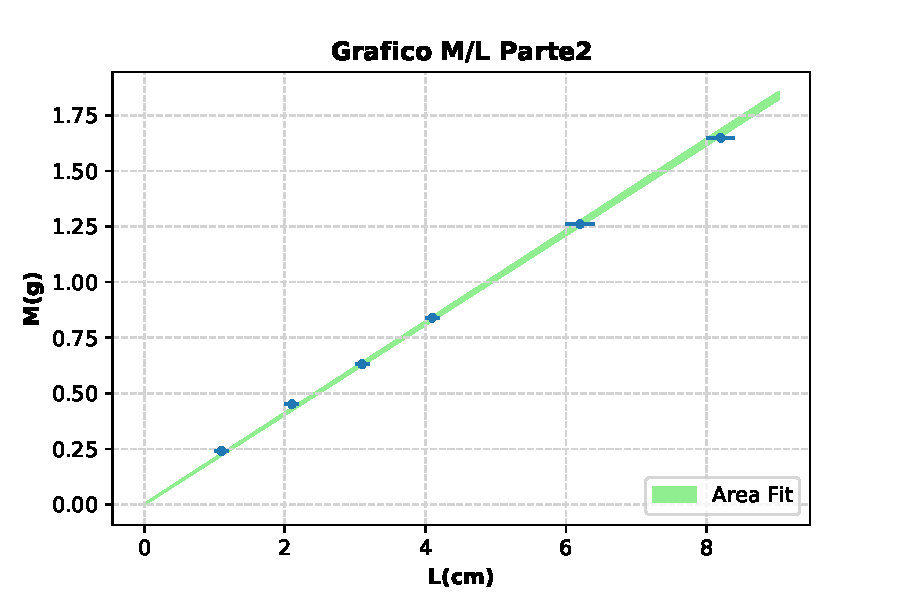
\includegraphics[width=13.5cm]{Figures/GraficoMLParte2.pdf}
  \caption{Grafico della differenza di massa in grammi in funzione della lunghezza del circuito stampato L in metri. La variazione di massa è stata ottenuta come differenza con la massa a circuito aperto e gli è stato attribuito un errore di $0.02g$ ottenuto da una somma diretta degli errori sulle singole pesate. I circuiti stampati erano percorsi da una corrente fissata di 3A. Per l'errore sulla lunghezza dei circuiti si è fatto riferimento al manuale come illustrato nella strumentazione. Si nota un andamento dei dati lineare compatibilmente con la formula [\ref{eq:FL}] e con il fit usato, della forma $M = pendenza \cdot L$ quindi passante per lo 0. L'area di fit è quella compresa tra le rette di massima e di minima pendenza.}   
  \label{fig:GraficoParteII}
\end{figure}
Da questo set di dati ci è stato possibile ricavare nuovamente il campo magnetico B del magnete A, facendo quindi una media pesata e calcolando la deviazione standard si è ottenuto il risultato:

\par
\begin{equation*}
    B_{SET3} = (6.9 \pm 0.3)\cdot 10^{-2}T
\end{equation*}
Questo valore di B e quelli calcolati nella parte I risultano compatibili tra di loro, è dunque possibile ottnere un valore finale del campo magnetico pari a:

\begin{equation*}
    B = (7.05 \pm 0.15)\cdot 10^{-2}T 
\end{equation*}

\par}